\section{Analysis of Social Network}\label{analysis-of-social-network}

\subsection{Introduction}
The relevance of social media and Graph Database
Characteristics of this kind of database.
The structure of the paper.

can 
\subsection{Objectives}\label{objectives}

The main goal of this research is to index information about social media metrics in a Graph Database (GDB), in order to discover relations and patterns inside the data. The question that has based this research is if and how a GDB can facilitate data analyses of social media metrics. Considering the 
characteristics of GDB and the nature of the information in social network, our hypothesis is that storing data in graphs enables us to have more accessible and understandable queries, in comparison to other methods of storing data such as SQL, files, and other usual ones.

\subsection{Methodology}

The metrics data from social network are indexed in a GDB, then some queries are performed in order to discover what patterns emerge. The GDB selected to be used is Neo4j\cite{}. Neo4j is the chosen one due to the model of graph (property graph), documentation available and for its free access (comunity edition). 

:::First findings (result of gdb)

\subsubsection{Workflow}\label{workflow}

\begin{figure}
\centering
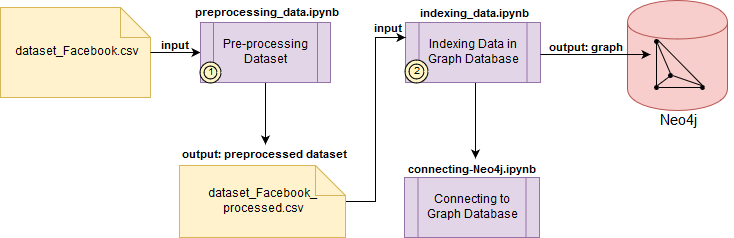
\includegraphics{../figures/research.png}
\caption{Research Workflow}
\end{figure}

\subsection{Description of data}\label{description-of-data}

The dataset used is available in
http://archive.ics.uci.edu/ml/datasets/Facebook+metrics. The dataset has
19 features and 500 instances.

\subsection{Methods}\label{methods}

Neo4j Graph Database will be used in this research. Neo4j has librarys
to be used in Python.

\subsection{Future Works}

To create further queries about data relations and patterns.
How data mining can be combined with GDB, based on the results of this research.

\subsection{References}\label{references}

S. Moro, P. Rita and B. Vala. Predicting social media performance
metrics and evaluation of the impact on brand building: A data mining
approach. Journal of Business Research, Elsevier, In press, 2016.
